% TeX root=../main.tex

\section{Descobrindo o luvita}

\emph{Luvita} denota um povo e uma língua e seus dialetos cuja existência,
até o começo do século passado, estava perdida na história.\footnote{Esta seção
	está baseada sobretudo em \textcite{CHLI11,Melchert2003,Hoffner2008}.}
Quando no final do século \textsc{xix} foram encontrados blocos de pedra no
norte da Síria com inscrições em hieróglifos em alto relevo, os arqueólogos associaram esta
nova língua e o povo que a escreveu com os \emph{hititas}, um povo que até
então era lembrado por passagens da bíblia hebraica e alguns documentos
recentemente descobertos em assírio.
Em 1906, as escavações realizadas em Boğazköy\slash{}Boğazkale sob direção de
Hugo Winckler e Theodore Makridi revelaram a cidade de Hattusa,
capital do que teria sido depois chamado de Império Hitita, e nela um grande
arquivo de documentos em cuneiforme em uma língua até então
desconhecida.\footnote{A decifração do cuneiforme nesta altura já estava
	bastante adiantada, tendo sido iniciada nos primeiros anos do século
	\textsc{xix} e relativamente bem estabelecida dentro da primeira metade do
	século para o persa antigo, acadiano e elamita.}
Apenas em 1915-17, Bedřich Hrozný conseguiria ao mesmo tempo demonstrar que a
língua nesses arquivos e em duas cartas previamente escavadas em
\href{https://pleiades.stoa.org/places/149576487}{Tell el-Amarna}
(Egito moderno) era uma língua indo-europeia e produzir um esboço gramatical
dela, identificando-a como a língua dos hititas.
Entre os textos em cuneiforme escavados em Boğazköy entre 1906 e 22 alguns revelaram
dentro deles trechos que os autores das tabuletas avisam que devem ser lidos
\emph{luwili}, isto é ``como luvita''.\footnote{Os códigos legais hititas
	contém provisões também de uma região, ainda hoje
	com localização disputada, chamada \mbox{\textsc{kur} \textit{Lu-ú-i-ya}}.}
Como alguns termos soltos ou incluídos em léxicos dessa língua
aparecem marcados com um sinal cuneiforme, \foreignlanguage{hittite}{𒃵}, chamado
pelo nome alemão \emph{Glossenkeil}, sugeriu-se chamar essa língua também de
\emph{Glossenkeilsprache}.\footnote{Os textos em luvita cuneiforme estão
	editados em~\textcites{Starke1985}{YakubovichMouton2023}.
	Outra língua aparece, embora raramente,
	nos textos hititas precedida por \foreignlanguage{hittite}{𒃵}, o palaico. Os
	textos em palaico estão editados em~\textcite{Carruba1970}.}

A língua dos hieróglifos das inscrições sírias, no entanto, permaneceu
praticamente ilegível desde sua descoberta até a década de 30.\footnote{Alguns
	sinais tinham sido corretamente interpretados por Sayce entre 1882 e 1884, a
	saber os logogramas \mbox{L.17 𔐑 \textsc{rex}} e \mbox{L.228 𔔆 \textsc{regio}},
	respectivamente correspondentes aos cuneiformes
	\mbox{\foreignlanguage{hittite}{𒈗} \textsc{lugal}} `rei' e \mbox{\foreignlanguage{hittite}{𒆳} \textsc{kur}}
	`país\slash{}território'.}
No começo da década de 30, contribuições separadas de Meriggi, Gelb, Forrer,
Bossert e Hrozný ofereceram interpretação de diversos logogramas e
interpretações ou, ao menos, aproximações para alguns silabogramas,
permitindo as primeiras tentativas de interpretação.
Alguns avanços foram feitos durante as décadas de 1940 a 1960, com a compilação
de selos digráficos (hieroglíficos e cuneiformes) e com a publicação parcial da
inscrição bilíngue em hieroglífico e fenício de Karatepe descoberta por
Bossert e Halet Çambel.
Foi apenas com a publicação das ``Novas leituras''
por~\textcite{HawkinsMorpurgoNeumann1974} que se pode finalmente identificar a
língua dos hieróglifos hititas com a língua dos
\emph{\foreignlanguage{german}{Glossenkeil}} que deveriam
ser lidos \emph{luwili}.
Daí em diante, estas línguas passaram a ser conhecidas respectivamente como
\emph{luvita hieroglífico} e \emph{luvita cuneiforme}.

\section{Quando e onde?}

Embora tenhamos contado um pouco sobre a descoberta e decifração do luvita
hieroglífico, convém dizer um pouco sobre o contexto histórico dessa língua.

\subsection{Datação}
A maioria das informações históricas sobre os falantes de luvita ou habitantes
das regiões da associadas à língua luvita advém de textos hititas, salvo algumas
poucas evidências contidas nas cartas de Amarna, correspondências em acadiano
entre governantes egípcios e governantes do oriente próximo, incluindo duas
entre o Egito e Arzawa, o nome tradicionalmente atribuído ao território dos
falantes de luvita.
Os primeiros textos legais hititas contendo menções à
terra chamada de \emph{Luwiya}, hit.\ \mbox{\textsc{kur} \textit{Lu-ú-i-ya}},
datam da metade do segundo milênio antes da era comum, no Velho Reinado
Hitita.\footnote{CTH 291 e 292. Tradução das leis em \textcite{Hoffner1997}.}
Pelas crônicas históricas, sabe-se que pelo menos desde o reinado de Hattusili I
(\emph{ca.} 1650--1620)\footnote{Usarei ao longo deste texto as datas de acordo
	com a cronologia média do oriente próximo.} já havia interações entre hititas
e luvitas.
Supõe-se deste~\textcite{Starke1985} que os textos em luvita cuneiforme tenham
sido compostos entre os séculos \textsc{xvi} e \textsc{xv} \textsc{aec}.
Quanto ao luvita hieroglífico, o corpus se divide tradicionalmente em dois
períodos, o período imperial e período neo-hitita.

\paragraph{Imperial \slash{} Era do Bronze} Datadas do séc.\ \textsc{xiii aec},
entre as dinastias de Tudhaliya IV e Suppiluliuma II, parte final do Império
hitita.
Boa parte das inscrições do período imperial fazem forte uso de logogramas,
de modo que são de pouco interesse linguístico e de difícil
compreensão.\footnote{Duas inscrições apenas contém logogramas, de modo que
	se pode supor que talvez representem um texto hitita, a saber BOĞAZKÖY 1 e 2.}
Além das inscrições, como em~\autoref{fig:bogazkoy21},
temos selos reais e oficiais
como~\autoref{fig:tarkondemos}.

\begin{figure}[htb]
	\begin{center}
		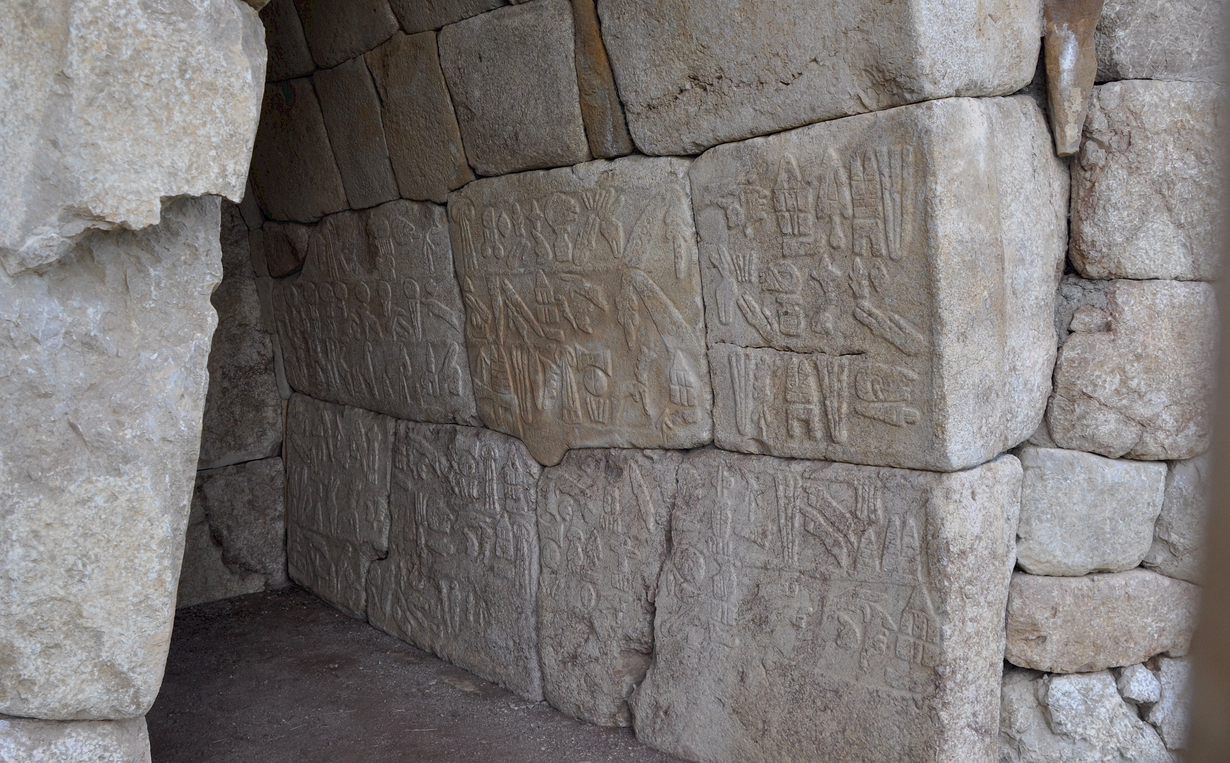
\includegraphics[width=\textwidth]{../../../Mídia/BOGAZKOY_21.jpg}
		\caption[Inscrição BOĞAZKÖY 21]{Inscrição BOĞAZKÖY 21. Dentro do complexo
			das piscinas sagradas de Hattusa, contendo o nome de Suppiluliuma II.\@
			Imagens de \href{https://www.hittitemonuments.com/bogazkoy/}{Hittite Monuments}.
			Ver~\citet[p. 48ff.]{CHLI3}
		}\label{fig:bogazkoy21}
	\end{center}
	\begin{center}
		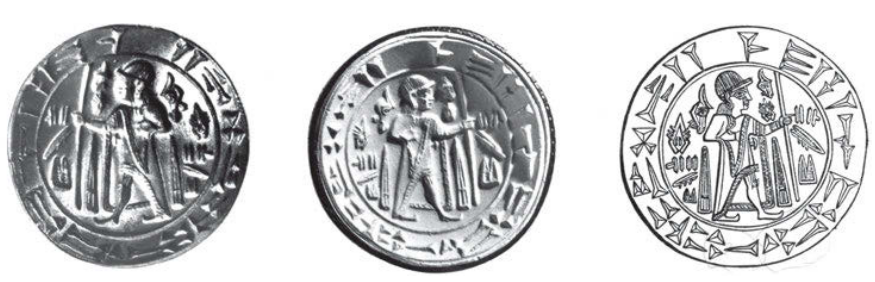
\includegraphics[width=\textwidth]{../../../Mídia/tarkondemos.png}
	\end{center}
	\caption[Selo de ``Tarkondemos'']{Selo de ``Tarkondemos''. Digráfico com
		cuneiforme na circunferência e hieróglifos no centro. Atualmente o texto é
		interpretado como pertencente a um certo \emph{Tarkas{(sa)}nawa}. Final do
		século \textsc{xii aec}. Atualmente em Walters Art Gallery, Baltimore,
		no. 57.1512. Imagem e traçado de~\citet[p. 45f.; \emph{plate} 32]{CHLI3}
	}\label{fig:tarkondemos}
\end{figure}

\paragraph{Neo-hitita \slash{} Era do Ferro} \emph{Circa} 1100-700 \textsc{aec},
período posterior à dissolução do império hitita que, aparentemente, foi
sucedido por diversas cidades-estado que mantiveram alguns aspectos
culturais e políticos do antigo império.
O corpus é composto sobretudo por inscrições, mas contém também selos,
como~\autoref{fig:lidar1}, e cartas, como~\autoref{fig:assur1}.

\begin{figure}[htb]
	\begin{center}
		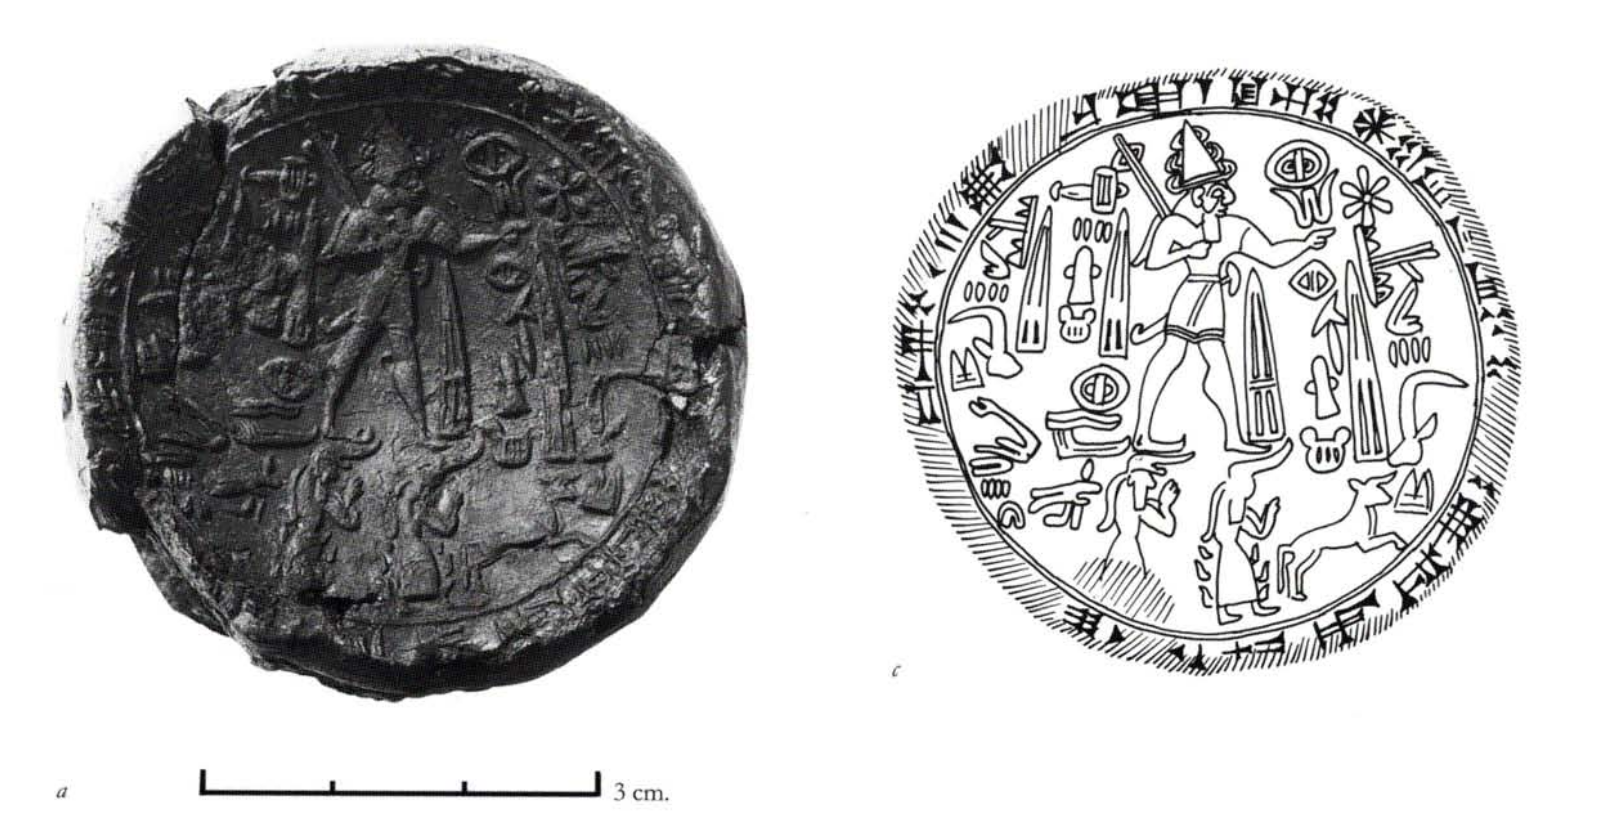
\includegraphics[width=\textwidth]{../../../Mídia/lidar1.png}
	\end{center}
	\caption[Bula de LİDAR]{Bula de LİDAR.\@ 5.4cm de diâmetro. Aproximadamente
		1200 \textsc{aec}. Atribuído a Kuzi-Tešub, rei de Carquemis.
		Atualmente no Şanlıurfa Arkeoloji Müzesi.
		Imagem e traçado de~\citet[\emph{plate} 328]{CHLI13}}\label{fig:lidar1}
	\begin{center}
		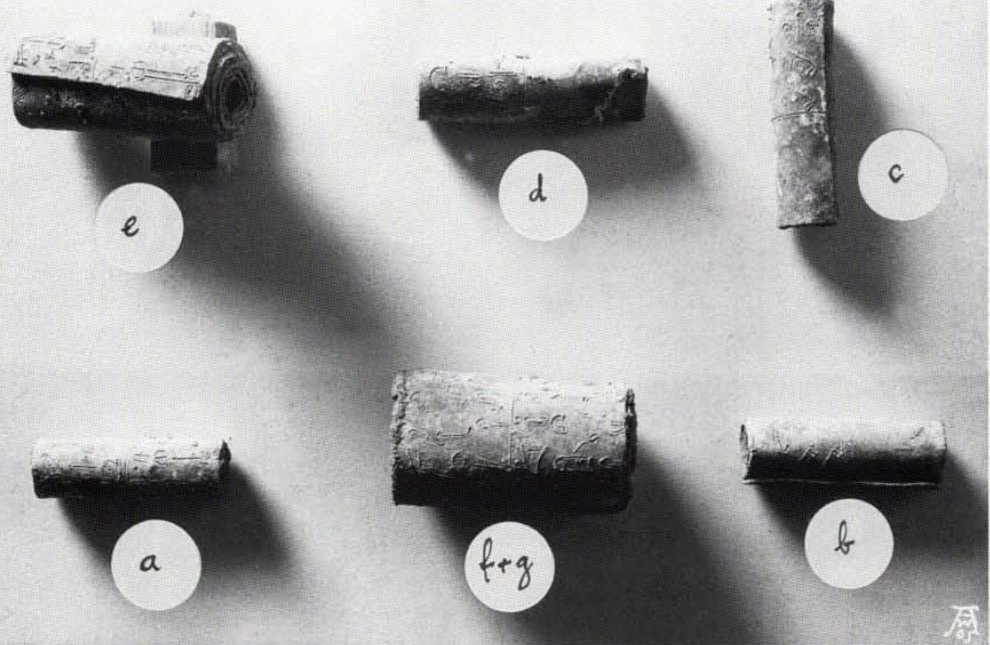
\includegraphics[width=\textwidth]{../../../Mídia/assur1.png}
	\end{center}
	\caption[Cartas de Assur]{Cartas de Assur. Rolos de chumbo de aproximadamente 4cm de altura e
		diversas larguras contendo cartas de comerciantes.
		Escavados em Assur em 1905 pela Deutsche Orientgesellschaft.
		Originalmente alocados no Eski Şark Eserleri Müzesi, apenas os
		fragmentos \emph{e} e \emph{f} estão preservados e locados no
		Vorderasiatisches Museum, Berlin, no. VA 5819.
		Imagem de~\citet[\emph{plate} 306]{CHLI13}
	}\label{fig:assur1}
\end{figure}

\clearpage

\subsection{Localização}

O mapa em~\autoref{fig:mapa1} mostra a localização de descoberta de todos os
documentos em luvita hieroglífico encontrados até hoje.
É de se notar que os documentos do período imperial hitita, em laranja no
mapa, estão muito mais espalhados geograficamente do que os documentos do
período neo-hitita, em verde, que se concentram sobretudo no sudeste da Anatólia
e noroeste da atual Síria.

\begin{figure}[ht!]
	\begin{center}
		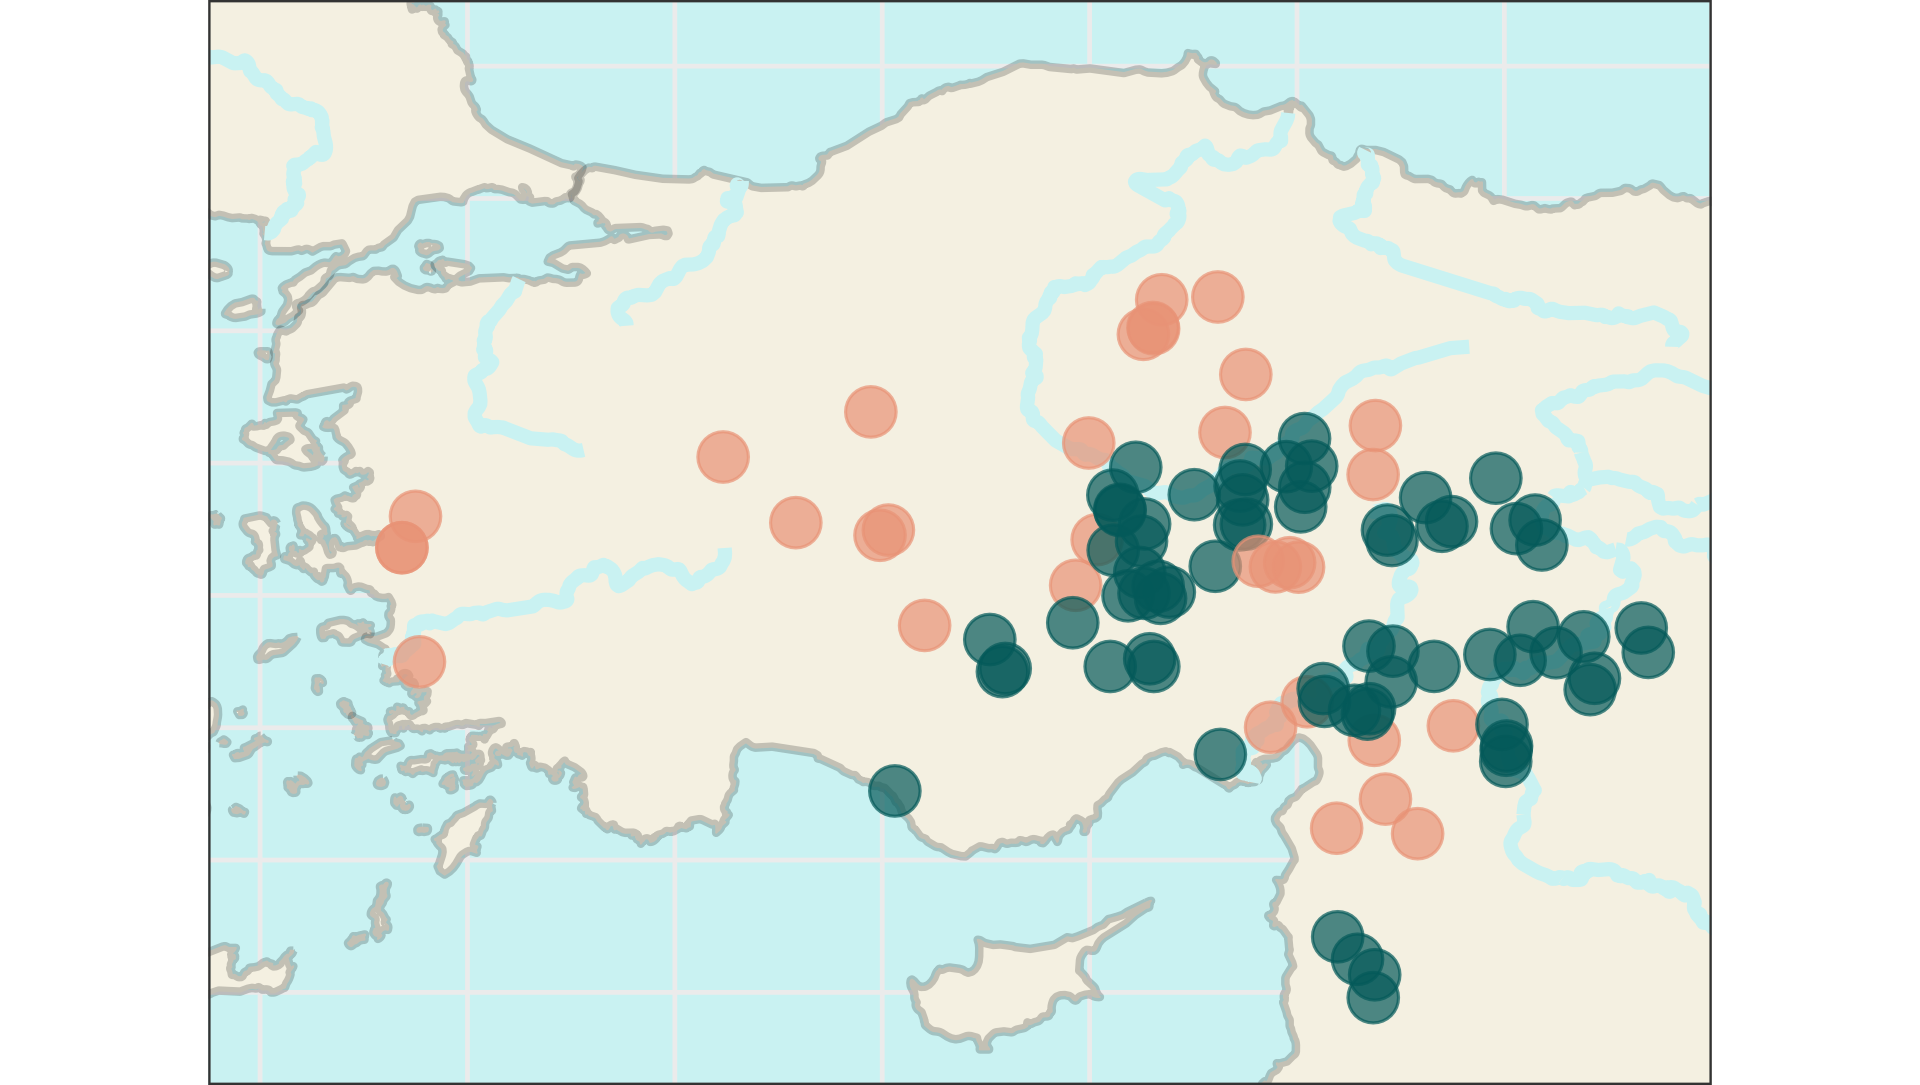
\includegraphics[width=1\textwidth]{../../../Mídia/Map01.png}
	\end{center}
	\caption[Mapa das inscrições monumentais]{Mapa contendo a localização das
		inscrições monumentais em luvita hieroglífico. Os pontos laranjas
		representam inscrições do período imperial enquanto os verdes, inscrições do
		período neo-hitita.}\label{fig:mapa1}
\end{figure}

\paragraph{Locais de interesse na idade do bronze}
As principais regiões que se assume terem sido ocupadas por falantes de luvita
durante a idade do bronze são Kizzuwatna, Tarhuntassa, Arzawa, Wilusa e,
possivelmente, Mira.
Todas essas regiões estão em volta do centro do poder hitita em Hatti, como se
pode ver no mapa em~\autoref{fig:mapa2}.

\paragraph{Locais de interesse na idade do ferro}
As principais regiões que se assume terem sido ocupadas por falantes de luvita
durante a idade do ferro são a Cilícia, Que e Gurgum.
Os sítios de Karatepe, Carquemis, Hama e Maraş estão entre os mais importantes.
Todas essas regiões estão entre o sudeste da atual Turquia e noroeste da Síria,
como se pode ver no mapa em~\autoref{fig:mapa3}.

\vfill
\clearpage

\begin{figure}[ht!]
	\begin{center}
		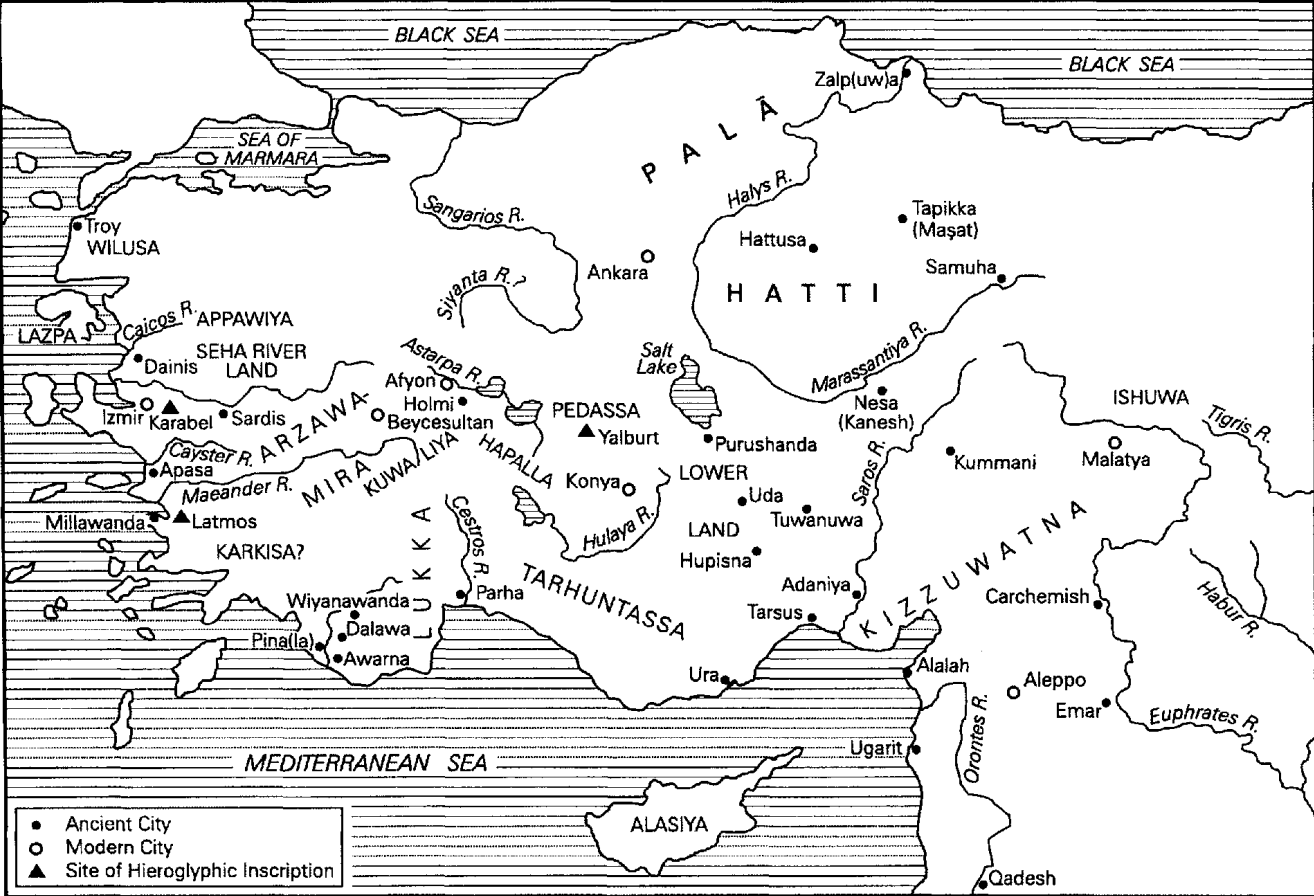
\includegraphics[width=0.95\textwidth]{../../../Mídia/Mapa02.png}
	\end{center}
	\caption[Mapa da Anatólia durante a idade do bronze]{Mapa da Anatólia durante
		a idade do bronze.~\citet[37]{Melchert2003}.}\label{fig:mapa2}
	\begin{center}
		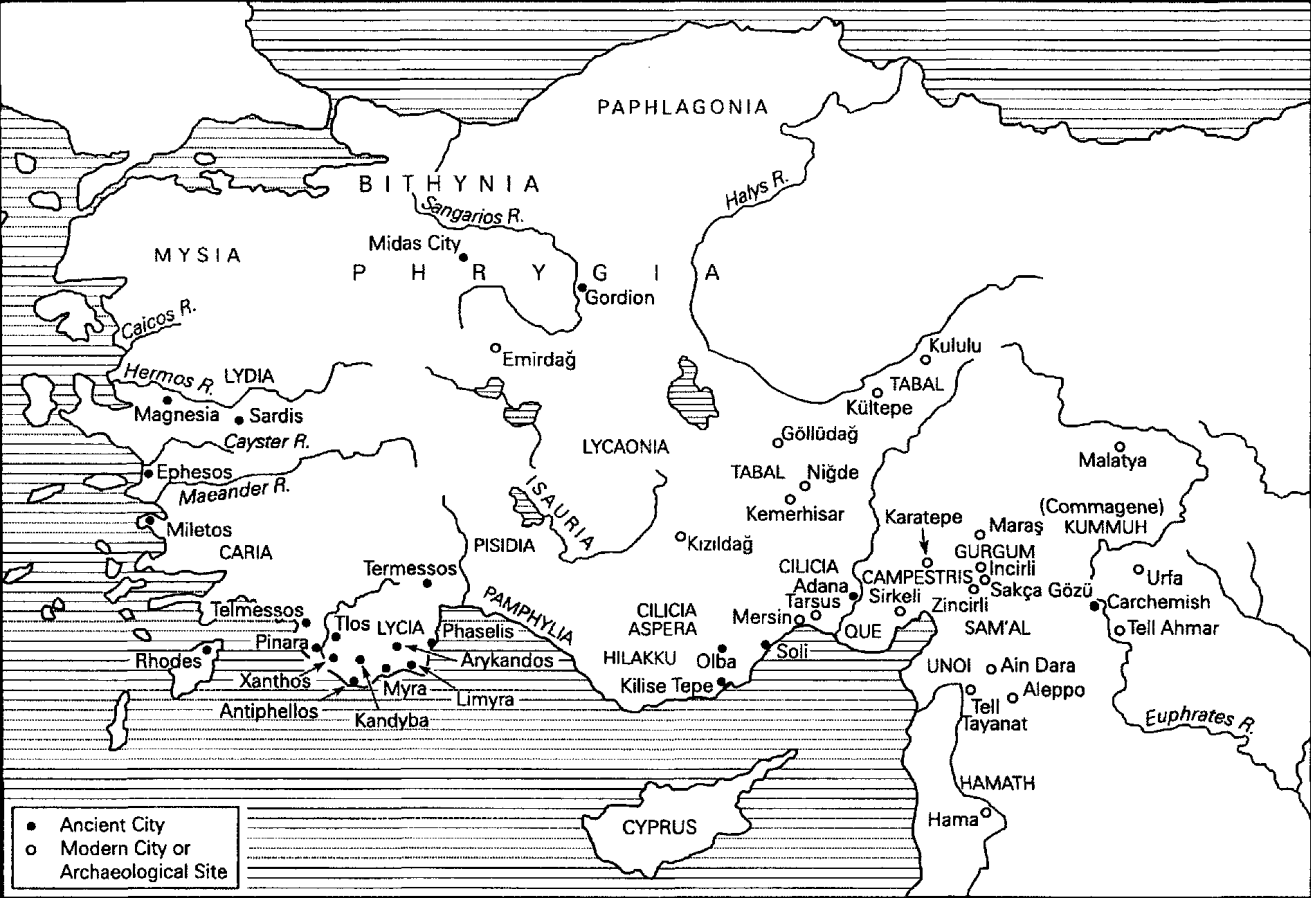
\includegraphics[width=0.95\textwidth]{../../../Mídia/Mapa03.png}
	\end{center}
	\caption[Mapa da Anatólia durante a idade do ferro]{Mapa da Anatólia durante
		a idade do ferro.~\citet[94]{Melchert2003}.}\label{fig:mapa3}
\end{figure}

\clearpage

\section{Parentesco linguístico}

O luvita é uma língua indo-europeia pertencente ao ramo anatólico.
O proto-indo-europeu (\textsc{pie}) é uma língua hipotética reconstruída a
partir da comparação entre línguas genealogicamente ligadas umas a outras
utilizando o método linguístico histórico comparativo.
As línguas mais importantes utilizadas para sua reconstrução desde o início do
século \textsc{xix} foram o sânscrito e o grego, em primeiro lugar, o latim, as
línguas germânicas e as balto-eslávicas, secundariamente, e as célticas,
o armênio e albanês, com menor frequência.
Com as evidências oferecidas por Bedřich Hrozný para a hipótese de que o
hitita seria uma língua indo-europeia, iniciou-se um processo de revisão do que
seria o proto-indo-europeu e qual sua relação com essa recém descoberta língua.
Desde cedo ficou claro que o hitita representava um destacamento bastante antigo
da língua indo-europeia que havia gerado os demais ramos.\footnote{Pelo menos
	desde~\citet{Sturtevant1933}.}
Com a decifração de línguas como o luvita, cário, palaico, lídio e lício chegou-se
à conclusão de que todas elas formam junto do hitita um ramo linguístico dentro do
indo-europeu, comumente chamado de ramo \emph{anatólico}.\footnote{Não cabe aqui
	a discussão se a separação do anatólico do resto do indo-europeu o torna um
	ramo ``de primeira classe'', pertencendo assim não ao indo-europeu, mas a uma
	língua que poderia ser chamada de indo-hitita \slash{} indo-anatólico,
	detalhes sobre essa discussão podem ser encontrados em~\citet{Ringue2017}.}

Dentro das anatólicas, uma divisão conservadora das línguas seria a proposta
por~\citet[305--6]{Rieken2017}:
\begin{inparaenum}
	\item do Anatólico ``Comum'' o hitita e palaico teriam se separado
	inicialmente;
	\item as demais línguas, i.e.\ o luvita, lício, lídio e cário seriam
	provenientes de um dialeto anatólico do Sul, um
	``anatólico meridional'', ou, em árvore genealógica:\footnote{Nestas e nas
		próximas árvores, os nódulos em itálico representarão estágios linguísticos
		não atestados, mas supostamente reconstruídos.}
\end{inparaenum}

\vspace{3pt}
\begin{center}
	\begin{tikzpicture}
		\Tree [.{\emph{Anatólico `Comum'}}
			Hitita
			Palaico
				[.{\emph{Anatólico `Meridional'}}
					Luvita
					Lício
					Lídio
					Cário
				]
		]
	\end{tikzpicture}
\end{center}

O modelo mais comumente aceito, no entanto, é o de~\citet[92]{Oettinger1978} e
seguido por~\citet[6]{Yakubovich2010}, que utiliza as seguintes isoglosas para a
divisão:
\begin{inparaenum}
	\item substituição da desinência de primeira pessoa singular presente ativa
	indoeuropeia *\emph{-mi} por \emph{-wi} em todas as línguas menos hitita;
	\item generalização da forma de primeira pessoa singular pretérita \emph{-ha}
	salvo em lídio;
	\item plural em formas derivadas em *\emph{-nsi} no lugar de *\emph{-es} em
	cário, lício e luvita.
\end{inparaenum}
Esquematicamente:

\begin{center}
	\begin{tikzpicture}
		\Tree [.{\emph{Anatólico `Comum'}}
		Hitita
		[.{\emph{Não-hitita}}
		Lídio
		[.{\emph{Lúvio-palaico}}
		Palaico
			[.{\emph{Lúvio}}
				Cário
				Lício
				Luvita
			]
		]
		]
		]
	\end{tikzpicture}
\end{center}

Por fim, embora seja comum dizer que o luvita registrado em cuneiforme e o
luvita registrado em hieróglifos correspondem a dialetos
distintos,~\citet{Yakubovich2010} apresenta evidências de que os
documentos cuneiformes luvitas representam dois dialetos contemporâneos
associados a regiões geográficas distintas: o dialeto de Kizzuwatna (sudeste da
atual Turquia) e o dialeto ``Imperial'', associado às regiões centrais do
império hitita.
Por sua vez, os textos em hieróglifos registrariam um dialeto sucessor do
dialeto ``Imperial'', que o autor chama de ``luvita da idade do ferro''.
As principais isoglosas utilizadas para defender essa organização são:
\begin{inparaenum}
	\item os textos associados a Kizzuwatna não registram formas de genitivo, mas
	sim de adjetivos possessivos em \emph{-assa-};
	\item também nos textos de Kizzuwatna, o morfema de imperfectivo \emph{-zza}
	é substituído pelo morfema \emph{-ssa}.
	\item os demais textos cuneiformes apresentam uma tendência a substituir o
	acusativo plural comum \emph{-anza} pela forma nominativa \emph{-anzi},
	os textos hieroglíficos jamais diferenciam nominativo de acusativo plural.
	\item os clíticos \emph{=pa} e \emph{=tar} parecem ter desaparecido nos textos
	hieroglíficos.
\end{inparaenum}


\begin{center}
	\begin{tikzpicture}
		\Tree [.{\emph{Luvita `Comum'}}
				{Luvita de Kizzuwatna}
				[.{Luvita ``Imperial''}
						{Luvita da Idade do Ferro}
				]
		]
	\end{tikzpicture}
\end{center}

\section{Recomendações bibliográficas}

Detalhes sobre a descoberta, publicação e decifração dos hieróglifos luvitas
podem ser encontrados em~\citet[pp. 131ff.]{HawkinsScripts}. Para uma descrição
ainda mais detalhada, recomenda-se~\citet[pp. 6-17]{CHLI11}.
O compêndio de~\citet{Melchert2003} oferece detalhes e bibliografia para todos
os aspectos da história, geografia e língua luvita.
Sobre a história do oriente próximo, incluindo os hititas, luvitas e sua
relações com outros povos da região, reco\-men\-da-se~\citet{Mieroop2015}, sobretudo
as seções 6.3, 8.2 e 11.1.
Informações detalhadas sobre as línguas anatólicas podem ser encontradas
em~\citet[239--308]{HSK41.1} e, sobre a dialetologia do luvita,
ver~\citet{Yakubovich2010}.
